\section*{Práctica 8 - Ejercicios para el final}

\subsection*{Ejercicio 1}

\paragraph{1.} Para armar el esquema de recursión estructural, primero tenemos que identificar los constructores:
\begin{itemize}
  \item \xtt{Nil}: toma 0 parámetros.
  \item \xtt{Tern a (AT a) (AT a) (AT a)}: toma 4 parámetros (una raíz y los 3 árboles hijos).
\end{itemize}

Por lo que, si asumimos que nuestro tipo de salida es \xtt{b}, el esquema \xtt{foldAT} va a recibir 3 parámetros:
\begin{itemize}
  \item Un \xtt{b}, que es el que devolvemos cuando el \xtt{AT a} es \xtt{Nil}.
  \item Y una función \xtt{f::a->b->b->b->b} que dada una raíz, y el resultado recursivo en los 3 árboles hijos, nos devuelve un \xtt{b}.
  \item El árbol \xtt{AT a} sobre el cual se va a hacer el \xit{fold}.
\end{itemize}

Entonces, la función queda:
\begin{lstlisting}[language=Haskell]
foldAT::b->(a->b->b->b->b)->AT a->b
foldAT base _ Nil = base
foldAT base f (Tern a izq cent der) = f a (recu izq) (recu cent) (recu der)
    where recu = foldAT base f
\end{lstlisting}

\paragraph{2.} El esquema de recursión primitiva es similar al anterior, pero en el paso recursivo tenemos acceso a cual es el árbol que estamos procesando.

\begin{lstlisting}[language=Haskell]
recAT::b->(AT a->b->b->b->b)->AT a->b
recAT base f Nil = base
recAT base f arbol@(Tern a izq cent der) = f arbol (recu izq) (recu cent) (recu der)
    where recu = recAT base f
\end{lstlisting}

\paragraph{3.} Usando recursión explicita tenemos que:

\begin{lstlisting}[language=Haskell]
esSubarbol::Eq a => AT a->AT a->Bool
esSubarbol Nil _ = True
esSubarbol uno otro@(Tern a izq cent der) = uno == otro || recu izq || recu cent || recu der
    where recu = esSubarbol uno
\end{lstlisting}

Notemos que en la definición necesitamos si o si el árbol ``otro'' ya que lo necesitamos para el caso en que el árbol ``uno'' no es es subArbol de izq, cent o der. Entonces, podemos reescribirla usando \xtt{recAT}:

\begin{lstlisting}[language=Haskell]
esSubarbol::Eq a => AT a->AT a->Bool
esSubarbol Nil _ = True
esSubarbol uno = recAT True (\otro recuIzq recuCent recuDer->uno == otro || recuIzq || recuCent || recuDer)
\end{lstlisting}

\todo{REVISAR}

\subsection*{Ejercicio 2}
\begin{lstlisting}[language=Haskell]
funcionizar::Eq a => [a]->[b]->a->Maybe b
funcionizar _ [] _ = Nothing
funcionizar [] _ _ = Nothing
funcionizar (x:xs) (y:ys) p | p == x = y
                            | otherwise = funcionizar xs ys p
\end{lstlisting}

\subsection*{Ejercicio 3}
\begin{lstlisting}[language=Haskell]
inversaAcotada::Eq b => (a->b)->[a]->b->Maybe a
inversaAcotada f dom = funcionizar (map f dom) dom
\end{lstlisting}

\subsection*{Ejercicio 4}
\paragraph{1.} Igual que en el Ejercicio 1, identificamos los constructores:
\begin{itemize}
  \item \xtt{Cte Float}: toma 1 parámetro.
  \item \xtt{Suma expr expr}: toma 2 parámetro.
  \item \xtt{Div expr expr}: toma 2 parámetro.
\end{itemize}

Si asumimos que nuestro tipo de salida es \xtt{b}, el esquema \xtt{foldExpr} va a recibir 4 parámetros:
\begin{itemize}
  \item Una función \xtt{f::Float->b}, que se va a usar cuando la \xtt{expr} es constante.
  \item Una función \xtt{g::b->b->b}, que se va a usar cuando la \xtt{expr} es una suma.
  \item Una función \xtt{h::b->b->b}, que se va a usar cuando la \xtt{expr} es una división.
  \item La \xtt{expr} sobre la cual se va a hacer el \xit{fold}.
\end{itemize}

Entonces, la función queda:
\begin{lstlisting}[language=Haskell]
foldExpr::(Float->b)->(b->b->b)->(b->b->b)->expr->b
foldExpr f _ _ (Cte x) = f x
foldExpr f g h (Suma e1 e2) = g (recu e1) (recu e2)
    where recu = foldExpr f g h
foldExpr f g h (Div e1 e2) = h (recu e1) (recu e2)
    where recu = foldExpr f g h
\end{lstlisting}

\paragraph{2.} Primero con recursión explicita
\begin{lstlisting}[language=Haskell]
eval::expr->Maybe (Float,String)
eval (Cte x) = Just (x, "")
eval (Suma e1 e2) =
    case (eval e1) of
      Nothing->Nothing
      Just (res1, traza1)->
        case (eval e2) of
          Nothing->Nothing
          Just (res2, traza2)->Just (res1 + res2, traza1 ++ traza2)
eval (Div e1 e2) =
    case (eval e1) of
      Nothing->Nothing
      Just (res1, traza1)->
        case (eval e2) of
          Nothing->Nothing
          Just (res2, traza2)->if res2 != 0 then Just (res1 / res2, traza1 ++ traza2) else Nothing
\end{lstlisting}

\paragraph{3.} Ahora usando \xtt{foldExpr}
\begin{lstlisting}[language=Haskell]
eval::expr->Maybe (Float,String)
eval = foldExpr (\x->Just (x, ""))
                (\r1 r2->
                  case r1 of
                    Nothing->Nothing
                    Just (res1, traza1)->
                      case r2 of
                        Nothing->Nothing
                        Just (res2, traza2)->Just (res1 + res2, traza1 ++ traza2))
                (\r1 r2->
                  case r1 of
                    Nothing->Nothing
                    Just (res1, traza1)->
                      case r2 of
                        Nothing->Nothing
                        Just (res2, traza2)->if res2 != 0 then Just (res1 / res2, traza1 ++ traza2) else Nothing)
\end{lstlisting}

\paragraph{4.} Nos dan como pista el tipo:
\begin{lstlisting}[language=Haskell]
data Evaluation = Ev (String->Maybe (Float,String))
\end{lstlisting}

Y el objetivo es poder definir \xtt{eval} como \xtt{eval expr = applyEv (evalM expr) ""}. Además, sabemos que:
\begin{lstlisting}[language=Haskell]
applyEv :: Evaluation -> String -> Maybe (Float, String)
applyEv (Ev f) s = f s
\end{lstlisting}

Y que \xtt{evalM::expr->Evaluation}.

Usando la técnica de los recuadros para abstraer las partes comunes entre \xtt{Suma} y \xtt{Div}, tenemos las siguientes funciones comunes:

\begin{lstlisting}[language=Haskell]
instance Monad Evaluation where
  -- return :: (String -> Maybe (Float, String) -> Evaluation
  return f = Ev f
  -- (>>=) :: Evaluation -> ((String -> Maybe (Float, String)) -> Evaluation) -> Evaluation
  (>>=) (Ev f) g = g f
\end{lstlisting}

Y las funciones específicas:

\begin{lstlisting}[language=Haskell]
liftM2 :: Monad m => (a -> b -> c) -> m a -> m b -> m c
liftM2 f mx my = do x <- mx
  y <- my
  return (f x y)

(</>) :: Monad m => m Float -> m Float -> m Float
(</>) = mx my = do
  x <- mx
  y <- my
  if y == 0 then Nothing else return (x/y)

(<+>) :: Monad m => m Float -> m Float -> m Float
(<+>) = liftM2 (+)
\end{lstlisting}

Con lo que ya podemos escribir

\begin{lstlisting}[language=Haskell]
evalM::expr->Evaluation
evalM (Cte x) = returnM (x, "")
evalM (Suma e1 e2) =
  evalM e1 >>= \v1 ->
  evalM e2 >>= \v2 ->
  return v1 <+> v2
evalM (Div e1 e2) =
  evalM e1 >>= \v1 ->
  evalM e2 >>= \v2 ->
  return v1 </> v2
\end{lstlisting}

\begin{lstlisting}[language=Haskell]
evalM::expr->Evaluation
evalM (Cte x) = returnM (x, "")
evalM (Suma e1 e2) =
  evalM e1 >>= \(r1, traza1) ->
  evalM e2 >>= \(r2, traza2) ->
  returnM (r1 + r2, traza1 ++ traza2)
evalM (Div e1 e2) =
  evalM e1 >>= \(r1, traza1) ->
  evalM e2 >>= \(r2, traza2) ->
  if r2 == 0
    then failM
    else returnM (r1 / r2, traza1 ++ traza2)
\end{lstlisting}

Que, agregandole \xit{syntatic sugar}, es lo mismo que:

\begin{lstlisting}[language=Haskell]
evalM::expr->Evaluation
evalM (Cte x) = returnM (x, "")
evalM (Suma e1 e2) = do
  v1 <- evalM e1
  v2 <- evalM e2
  return v1 <+> v2
evalM (Div e1 e2) = do
  v1 <- evalM e1
  v2 <- evalM e2
  return v1 </> v2
\end{lstlisting}

\begin{lstlisting}[language=Haskell]
evalM::expr->Evaluation
evalM (Cte x) = returnM (x, "")
evalM (Suma e1 e2) = do
  (r1, traza1) <- evalM e1
  (r2, traza2) <- evalM e2
  returnM (r1 + r2, traza1 ++ traza2)
evalM (Div e1 e2) = do
  (r1, traza1) <- evalM e1
  (r2, traza2) <- evalM e2
  if r2 == 0
    then failM
    else returnM (r1 / r2, traza1 ++ traza2)
\end{lstlisting}

\begin{lstlisting}[language=Haskell]
evalM (Cte x) = returnM x
evalM (Div e1 e2) = do
  v1 <- evalM e1
  v2 <- evalM e2
  return v1 </> v2
\end{lstlisting}

\subsection*{Ejercicio 5} Sin usar \xtt{fix}, tenemos:
\begin{lstlisting}[language=Haskell]
iterate::(a->a)->a->[a]
iterate sig base = base:(ite sig (sig base))
\end{lstlisting}

Por lo que con \xtt{fix}:
\begin{lstlisting}[language=Haskell]
fix :: (a -> a) -> a
fix f = f (fix f)

iterate::(a->a)->a->[a]
iterate = fix (\rec sig base -> base:(rec sig (sig base)))
\end{lstlisting}

\subsection*{Ejercicio 6} Cuando definimos una extensión del Cálculo $\lambda$ tenemos que definir:
\begin{itemize}
  \item Expresiones válidas
  \item Tipos
  \item Reglas de tipado
  \item Valores
  \item Reglas de semántica
\end{itemize}

Las expresiones que nos plantea el enunciado son:

\[M ::= \dots \vert raise_\sigma\ M \vert try\ M_1, M_2, \dots, M_n\ with\ N\]

Y nos dicen que los valores no se modifican.

Entonces, como nos dicen que las expresiones $M_1, M_2, \dots, M_n$ podrían dar error, agregamos a los tipos:

\[\sigma ::= \dots \vert Try_\sigma \vert Error_\sigma\]

Las nuevas reglas de tipado son:

\[\deriv{\Gamma \rhd M : Nat}{\Gamma \rhd raise_\sigma M : Error_\sigma}{T-Raise}\]

\[\deriv{\Gamma \rhd N : Nat \to \rho\quad \Gamma \rhd M_i : Try_{\sigma_i}\text{, con $1 \leq i \leq n$}}{\Gamma \rhd try\ M_1, M_2, \dots, M_n\ with\ N : \sigma_n}{T-Raise}\]

Y las reglas de semántica:

\[\deriv{}{try\ V_1, \dots, V_n\ with\ N \to V_n}{E-NoError}\]

\[\deriv{M_i \to M_i'}{try\ V_1, \dots, M_i ,\dots, M_n\ with\ N \to try\ V_1, \dots, M_i' ,\dots, M_n\ with\ N}{E-UnPaso}\]

\[\deriv{M_i \to raise_\sigma T}{try\ V_1, \dots, M_i ,\dots, M_n\ with\ N \to N\ T}{E-Error}\]

\todo{REVISAR}

\subsection*{Ejercicio 7}

Claramente queremos hacer algo como

\[pred \eqdef \lambda n : Nat. if iszero(n) then 0 else search (\lambda x: Nat. succ(y) == x)\]

donde usamos el search para buscar el Nat anterior a n. El único problema es definir el predicado de igualdad entre Nat (==), ya que necesitaríamos usar pred, que es la que estamos definiendo.

\todo{REVISAR}

\subsection*{Ejercicio 8} La extensión básica de listas consiste en:

\todo{Agregar algunas partes del ejercicio 17, práctica 2}

Para ayudarnos, vamos a escribir primero el map usando el fix, pero en Haskell:

\begin{lstlisting}[language=Haskell]
fix :: (a -> a) -> a
fix f = f (fix f)

map :: (a->b) -> [a] -> [b]
map = fix (\rec f l -> case l of
              [] -> []
              (x:xs) -> (f x):(rec f xs))
\end{lstlisting}

Entonces, lo traducimos a cálculo lambda:

\[map_{\sigma,\tau} \eqdef fix\ (\abs{rec}{\rho\to\rho}{\abs{f}{\sigma\to\tau}{\abs{l}{[\sigma]}{case\ l\ of\ \{[] \to [] \vert h::t \to (f\ h)::((rec\ f)\ t)\}}}}) \]

\todo{Revisar el tipo de rec}

\subsection*{Ejercicio 9}

\[\w{let\ x = U\ in\ V} = \Gamma \rhd S(let\ x = M\ in\ N')\]

donde,

\begin{itemize}
  \item $\w{U} = \Gamma_1 \rhd M : \tau$
  \item $\w{\sust{V}{x\from U}} = \Gamma_2 \rhd N: \sigma$
  \item $S = MGU(\{\sigma_1 \uni \sigma_2 \vert x:\sigma_1 \in \Gamma_1, x:\sigma_2 \in \Gamma_2\}$
  \item $N' = copiarAnotaciones(V,N)$
  \item $\Gamma = S\Gamma_1 \cup S\Gamma_2$
\end{itemize}

\xit{Notar} que $N'$ y el predicado $copiarAnotaciones$ son necesarios porque el $N$ inferido es el que tiene la $x$ reemplazada por $U$. Si directamente usamos $N$ en la respuesta no sólo estamos anotando los tipos, sino también modificando la expresión.

\todo{Falta usar el algoritmo nuevo con unos casos}

\subsection*{Ejercicio 10}

\todo{Usar el algoritmo del ejercicio 9 en algunos casos}

\subsection*{Ejercicio 11}

\todo{TODO}

\subsection*{Ejercicio 12}

\todo{TODO}

\subsection*{Ejercicio 13}

\paragraph{a.}

\[\w{U\ V} = \Gamma \rhd S(M\ N)\]

donde,

\begin{itemize}
  \item $\w{U} = \Gamma_1 \rhd M : \tau$
  \item $\w{V} = \Gamma_2 \rhd N : \rho$
  \item $t$ y $s$ variables frescas, tales que $s <: \rho$
  \item $S = MGU(\{\tau \uni s\to t\} \cup \{\sigma_1 \uni \sigma_2 \vert x:\sigma_1 \in \Gamma_1, x:\sigma_2 \in \Gamma_2\}$
  \item $\Gamma = S\Gamma_1 \cup S\Gamma_2$
\end{itemize}

\todo{Revisar}

\paragraph{b.}

\todo{aplicar el algoritmo del punto a}

\subsection*{Ejercicio 14}

\paragraph{1.}

Pasar $\forall x\forall y\exists z (P(x,z)\land P(y,z))$ a Forma normal de Skolem. Por pasos:

\begin{itemize}
  \item Forma normal negada: idem.
  \item Forma prenexa: idem.
  \item Forma normal de Skolem: $\forall x\forall y (P(x,f(x,y))\land P(y,f(x,y)))$
\end{itemize}

\paragraph{2.}

Pasar $\forall x\forall y((\exists z (P(x,z))\land (\exists z P(y,z))))$ a Forma normal de Skolem. Por pasos:

\begin{itemize}
  \item Forma normal negada: idem.
  \item Forma prenexa: $\forall x\forall y\exists w\exists v (P(x,w)\land P(y,v))$.
  \item Forma normal de Skolem: $\forall x\forall y (P(x,f(x,y))\land P(y,g(x,y)))$
\end{itemize}

\subsection*{Ejercicio 15}

\paragraph{a.} ¿Cuál es la relación entre el árbol de resolución y el árbol de búsqueda de Prolog?

El árbol de resolución sólo contiene los resultados exitosos que se van encontrando en el árbol de búsqueda.

En este sentido, el árbol de resolución equivale a una refutación, mientras que el árbol de búsqueda utiliza las reglas de búsqueda y selección de prolog para ir explorando las soluciones mediante \xit{backtracking}.

\todo{REVISAR}

\paragraph{b.} ¿Qué hay que verificar antes de llamar al algoritmo mgu para unificar dos cláusulas?

Hay que verificar que no compartan variables. Si este es el caso, hay que hacer un renombre de variables.

\todo{REVISAR}

\paragraph{c.} Calcular el resolvente entre las siguientes cláusulas: $\{P (x, y)\}, \{\lnot P (y, f (y))\}$.

Primero renombramos a $\{P (x, w)\}, \{\lnot P (y, f (y))\}$.

Luego, el resolvente es $\square$ usando $\{x\from y, w\from f(y)\}$.

\subsection*{Ejercicio 16}

Nuestra base de conocimientos:

\begin{enumerate}
  \item \xtt{a(U,0,U)}
  \item \xtt{a(X,s(Y),s(Z)):-a(X,Y,Z)}
\end{enumerate}

Nuestro goal: \xtt{a(s(0),V,s(s(0)))}

\paragraph{a.}
\begin{center}
  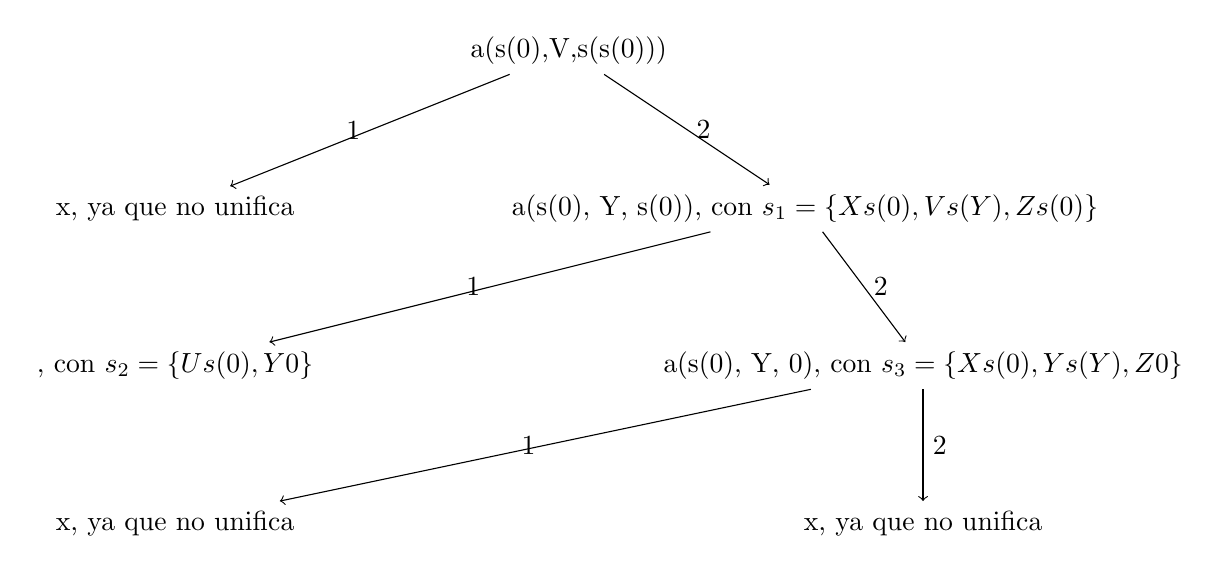
\begin{tikzpicture}
      \tikzstyle{ann} = [draw=none,fill=none,right]
      \node[draw=none, fill=none] (1a) at (0,0) {\xtt{a(s(0),V,s(s(0)))}};
      \node[draw=none, fill=none] (2a) at (-5,-2) {\todo{x}, ya que no unifica};
      \node[draw=none, fill=none] (2b) at (3,-2) {\xtt{a(s(0), Y, s(0))}, con $s_1=\{X\from \text{s(0)}, V\from \text{s(Y)}, Z\from \text{s(0)}\}$};
      \node[draw=none, fill=none] (3a) at (-5,-4) {$\square$, con $s_2=\{U\from s(0), Y\from 0\}$};
      \node[draw=none, fill=none] (3b) at (4.5,-4) {\xtt{a(s(0), Y, 0)}, con $s_3=\{X\from \text{s(0)}, Y\from \text{s(Y)}, Z\from \text{0}\}$};
      \node[draw=none, fill=none] (4a) at (-5,-6) {\todo{x}, ya que no unifica};
      \node[draw=none, fill=none] (4b) at (4.5,-6) {\todo{x}, ya que no unifica};
      \path [->](1a) edge node[left] {1} (2a);
      \path [->](1a) edge node[right] {2} (2b);
      \path [->](2b) edge node[left] {1} (3a);
      \path [->](2b) edge node[right] {2} (3b);
      \path [->](3b) edge node[left] {1} (4a);
      \path [->](3b) edge node[right] {2} (4b);
  \end{tikzpicture}
\end{center}

Luego, nos queda una sola sustitución resultado: $s = s_2 \circ s_1 = \{X\from \text{s(0)}, V\from \text{s(0)}, Z\from \text{s(0)}, U\from s(0)\}$, con lo que nuestra única solución es $V= s(0)$.

\paragraph{b.}

La base de conocimientos pasadas a cláusulas:
\begin{enumerate}
  \item $\{a(U,0,U)\}$
  \item $\{\lnot a(X,Y,Z), a(X,s(Y),s(Z))\}$
\end{enumerate}

El goal pasado a cláusula: $\{\lnot a(s(0),V,s(s(0)))\}$. Entonces,

\begin{itemize}
  \item Por 2, con $s_1=\{X\from \text{s(0)}, V\from \text{s(Y)}, Z\from \text{s(0)}\}$, tenemos la cláusula $4 = \{\lnot a(s(0), Y, s(0))\}$.
  \item Por 1, con $s_2=\{U\from s(0), Y\from 0\}$, tenemos la cláusula $\square$.
\end{itemize}

\subsection*{Ejercicio 17}

Seguimiento de \xtt{(c2 new) m3.}

\begin{tabular}{| c | c | c |}
  receptor & mensaje & resultado \\ \hfill
  C2 & new (de C2) & unC2 \\
  C2 & new (de C1) & unC2 \\
  C2 & new (de Object) & unC2 \\
  unC2 & m3 & 23 \\
  unC2 & m1 (de C1) & 23 \\
  unC2 & m2 (de C2) & 23 \\
\end{tabular}

\subsection*{Ejercicio 18}
